\documentclass[10pt,twocolumn]{article}
\usepackage{times}
\usepackage{spverbatim}
\usepackage[swedish]{babel}
\usepackage[utf8]{inputenc}
\usepackage{listings}
\usepackage[toc,page]{appendix}
\usepackage{graphicx}
\usepackage{mathtools}
\usepackage{float}
\usepackage{algorithm}
\usepackage{algpseudocode}
\usepackage[margin={2.45cm, 2.45cm}]{geometry}
\renewcommand\appendixname{Bilagor}
\renewcommand\appendixpagename{Bilagor}
\usepackage[compact]{titlesec}
\titlespacing{\section}{0pt}{*2}{*2}
\raggedbottom
\sloppy

\title{Lab 4\\ \emph{ModelView and ITAC}}

\author{Martin Söderén \\ marso329, 9009291098 }

\date{\today}

\begin{document}

\maketitle

\clearpage

\section{Introduction}

This lab consists of trying out a couple of different tools for debugging and optimizing parallel programs. The two different tools are TotalView and Intel Trace Analyzer and Collector (ITAC). 
\section{Method}
\subsection{TotalView}
There where some troubles getting TotalView to work in the NSC environment. The documentation for which modules to load where not updated so in the end I just used the buildenv-intel/2015-1 and the totalview/8.11.0-install0 modules to compile and run OpenMPI programs with TotalView. I had problems starting multiple TotalView after another, it complained that mpprun got incorrent arguements so I had to restart the session efter each run.  
I also had troubles with that it automatically breaked in MPI\_init but that was just a inconvenience.

\begin{figure}[H]
	\begin{center}
		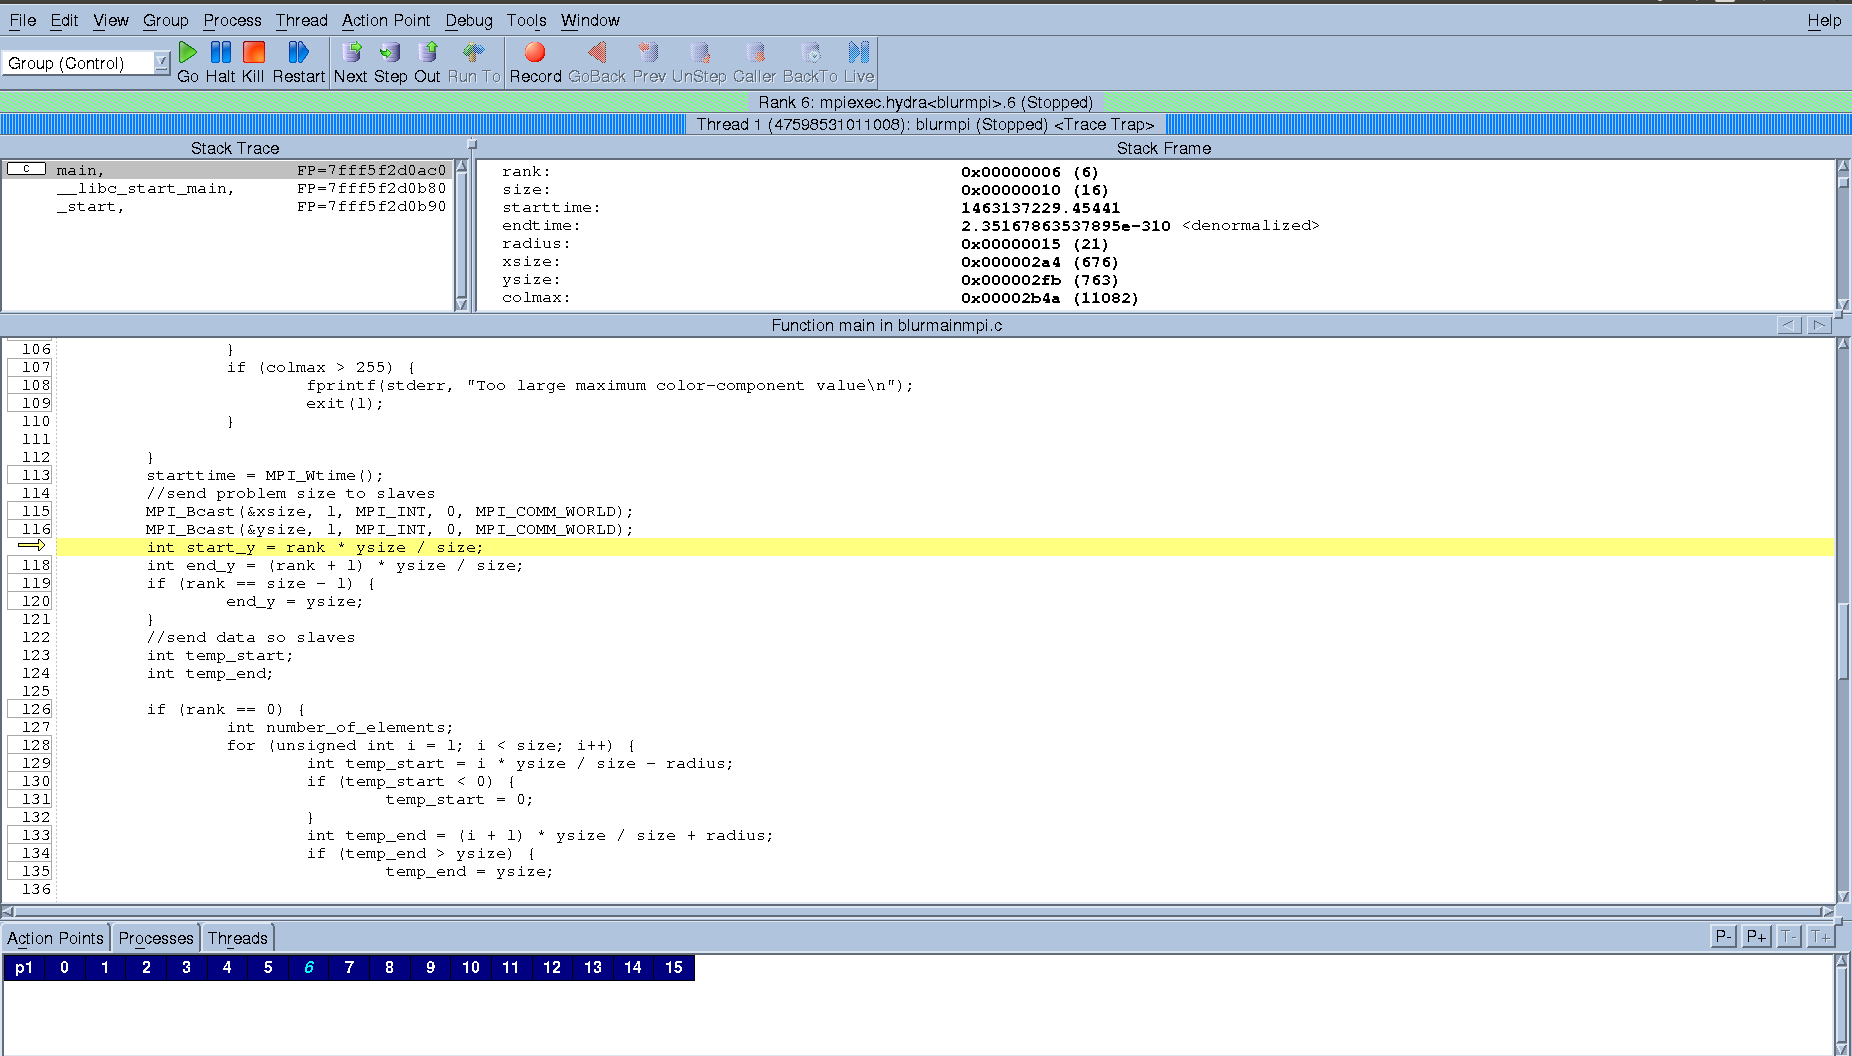
\includegraphics[scale=0.124]{figurer/screen.png}
	\end{center}
	\caption{Screen shoot of ModelView Usage}
\end{figure}
I "debugged" my blur filter from lab 1 by inserting a segmentation fault in the program.
\begin{lstlisting}[language=c]
	int* temp_int=0;
	int stupid=*temp_int;
\end{lstlisting}
By running the program with ModelView it caught the error and stopped the program. 
\begin{figure}[H]
	\begin{center}
		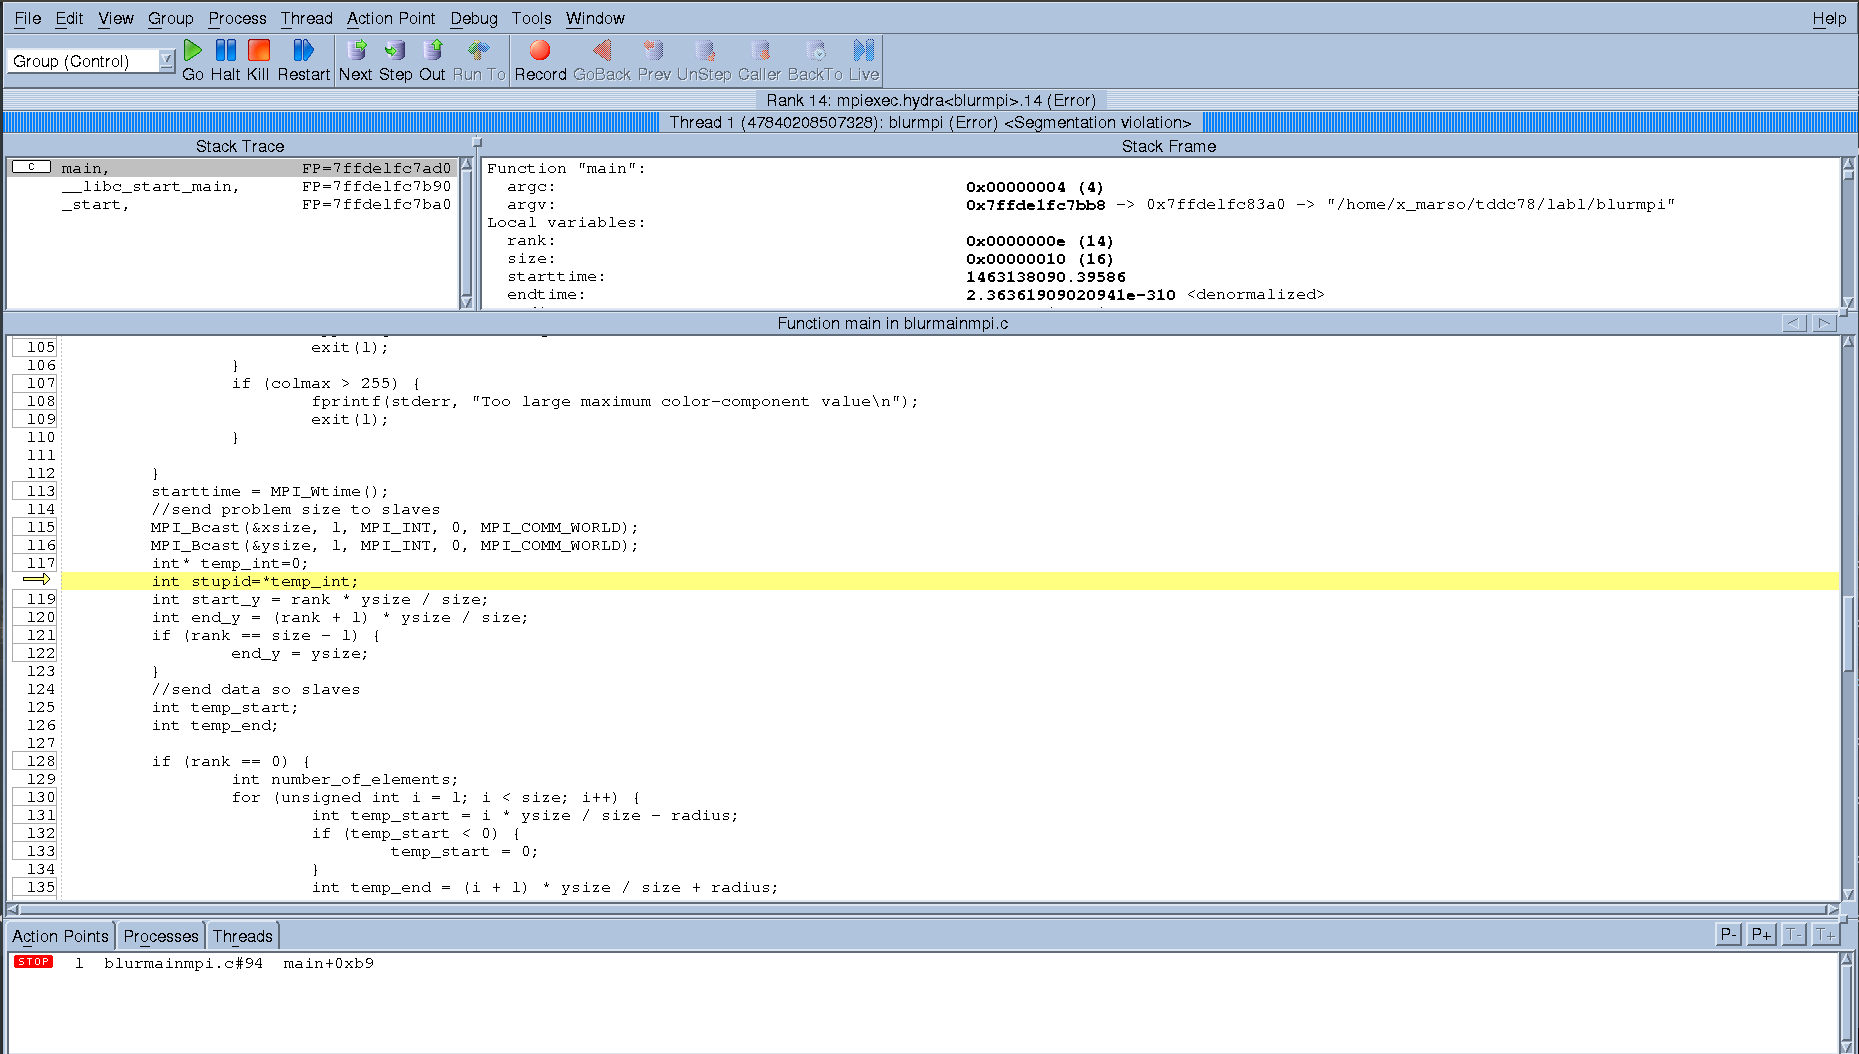
\includegraphics[scale=0.124]{figurer/screen1.png}
	\end{center}
	\caption{Screen shoot of ModelView Usage}
\end{figure}

Normally I use DDD when I debug programs and I noticed that you can't run DDD the normal way with DDD mpirun ./blurmpi 21 im1.ppm output.ppm since it will attach to the mpirun process. You can however start the process and then latter attach DDD to that process by finding its processid. That is however quite tedious and since the segmentation fault arises almost instantaneous you don't have time to attach DDD. So ModelView is good in that way with direct support for MPI programs. I also like how it displays local variables and arrays. Much better than DDD.

\subsection{ITAC}
I used ITAC on my code for blur filter in lab 1 and collected data. First I ran it with radius 21 as previous but all the trace data combined with the data in the calculation made my program exceed my disk quota so I reduced the radius to 4. I used VT\_classdef() and VT\_enter{} to see when each process entered and leaved the blurfiltermpi function which does the heavy calculation. From the traced I managed to see that my main thread does its work at the same time that the other threads are waiting for the data and then it sits for a long time waiting for the other threads to send back their data. This could be done more efficient by making the main threads part larger than the other threads so it has to do more work. 
\begin{figure}[H]
	\begin{center}
		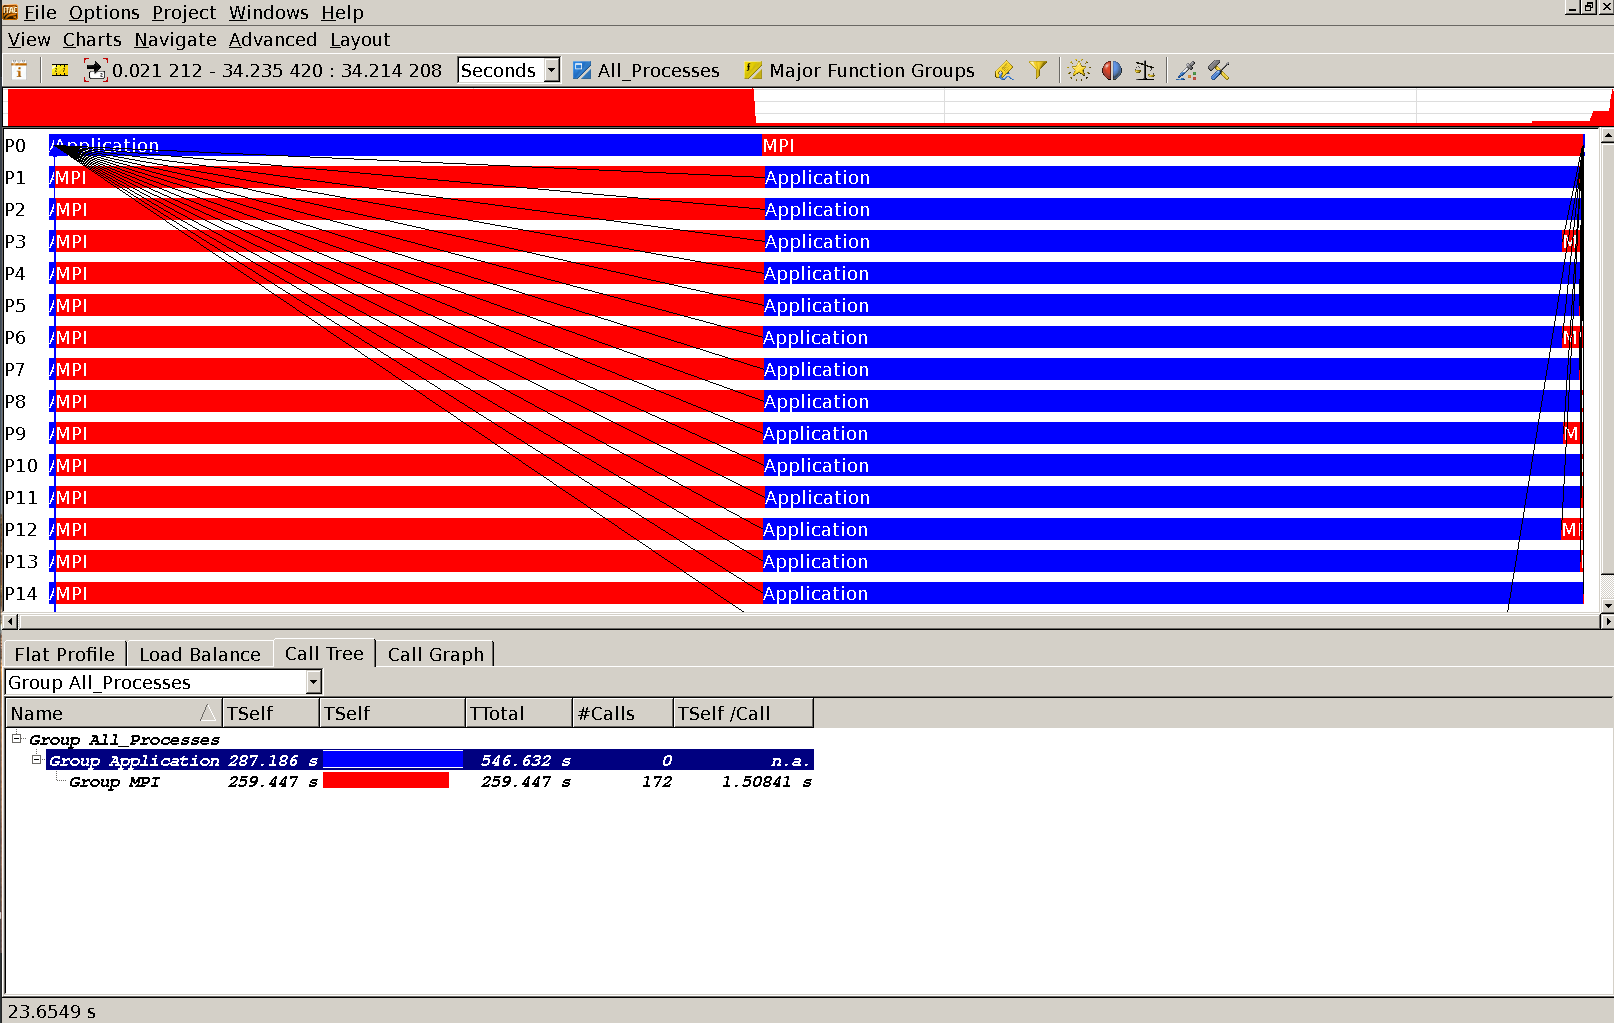
\includegraphics[scale=0.13]{figurer/screen2.png}
	\end{center}
	\caption{Screen shoot of ITAC}
\end{figure}

\section{Result}
Both programs works well and for debugging parallel programs I would say that ModelView is better than DDD, at least for MPI programs. DDD works well with Pthreads. ITAC is a good program for optimizing parallel programs without any doubt. I like the nice visualization options it features, for example a simple timeline of the program run. 



\end{document}
